\documentclass[14pt]{extbook}
\usepackage{multicol, enumerate, enumitem, hyperref, color, soul, setspace, parskip, fancyhdr} %General Packages
\usepackage{amssymb, amsthm, amsmath, bbm, latexsym, units, mathtools} %Math Packages
\everymath{\displaystyle} %All math in Display Style
% Packages with additional options
\usepackage[headsep=0.5cm,headheight=12pt, left=1 in,right= 1 in,top= 1 in,bottom= 1 in]{geometry}
\usepackage[usenames,dvipsnames]{xcolor}
\usepackage{dashrule}  % Package to use the command below to create lines between items
\newcommand{\litem}[1]{\item#1\hspace*{-1cm}\rule{\textwidth}{0.4pt}}
\pagestyle{fancy}
\lhead{Progress Quiz 2}
\chead{}
\rhead{Version A}
\lfoot{7862-5421}
\cfoot{}
\rfoot{Spring 2021}
\begin{document}

\begin{enumerate}
\litem{
Solve the equation below. Then, choose the interval that contains the solution.\[ -19(11x -10) = -3(13x -18) \]\begin{enumerate}[label=\Alph*.]
\item \( x \in [0.98, 1.12] \)
\item \( x \in [-1.65, -1.25] \)
\item \( x \in [1.37, 1.6] \)
\item \( x \in [0.74, 0.91] \)
\item \( \text{There are no real solutions.} \)

\end{enumerate} }
\litem{
Find the equation of the line described below. Write the linear equation as $ y=mx+b $ and choose the intervals that contain $m$ and $b$.\[ \text{Perpendicular to } 5 x - 8 y = 11 \text{ and passing through the point } (9, -6). \]\begin{enumerate}[label=\Alph*.]
\item \( m \in [-2.1, -0.83] \hspace*{3mm} b \in [8.4, 9.4] \)
\item \( m \in [-1.19, 0.25] \hspace*{3mm} b \in [8.4, 9.4] \)
\item \( m \in [-2.1, -0.83] \hspace*{3mm} b \in [-11.4, -5.4] \)
\item \( m \in [1.04, 1.72] \hspace*{3mm} b \in [-24.4, -19.4] \)
\item \( m \in [-2.1, -0.83] \hspace*{3mm} b \in [-19, -13] \)

\end{enumerate} }
\litem{
Find the equation of the line described below. Write the linear equation as $ y=mx+b $ and choose the intervals that contain $m$ and $b$.\[ \text{Perpendicular to } 9 x - 5 y = 7 \text{ and passing through the point } (9, -6). \]\begin{enumerate}[label=\Alph*.]
\item \( m \in [-0.89, -0.22] \hspace*{3mm} b \in [-17.2, -13.8] \)
\item \( m \in [-0.89, -0.22] \hspace*{3mm} b \in [-1.6, 0.6] \)
\item \( m \in [-2.82, -1.63] \hspace*{3mm} b \in [-1.6, 0.6] \)
\item \( m \in [-0.89, -0.22] \hspace*{3mm} b \in [0.5, 1.1] \)
\item \( m \in [-0.05, 1] \hspace*{3mm} b \in [-11.9, -9.5] \)

\end{enumerate} }
\litem{
First, find the equation of the line containing the two points below. Then, write the equation as $ y=mx+b $ and choose the intervals that contain $m$ and $b$.\[ (4, -11) \text{ and } (-9, -4) \]\begin{enumerate}[label=\Alph*.]
\item \( m \in [-2.3, -0.5] \hspace*{3mm} b \in [7.85, 10.85] \)
\item \( m \in [-2.3, -0.5] \hspace*{3mm} b \in [-24, -9] \)
\item \( m \in [-2.3, -0.5] \hspace*{3mm} b \in [-11.85, -6.85] \)
\item \( m \in [0.1, 4] \hspace*{3mm} b \in [-1.15, 1.85] \)
\item \( m \in [-2.3, -0.5] \hspace*{3mm} b \in [2, 6] \)

\end{enumerate} }
\litem{
Solve the linear equation below. Then, choose the interval that contains the solution.\[ \frac{-3x + 5}{3} - \frac{-5x + 3}{4} = \frac{4x -7}{6} \]\begin{enumerate}[label=\Alph*.]
\item \( x \in [-0.4, 1.6] \)
\item \( x \in [3.9, 5.1] \)
\item \( x \in [20, 22.4] \)
\item \( x \in [7, 9.4] \)
\item \( \text{There are no real solutions.} \)

\end{enumerate} }
\litem{
Write the equation of the line in the graph below in Standard form $Ax+By=C$. Then, choose the intervals that contain $A, B, \text{ and } C$.
\begin{center}
    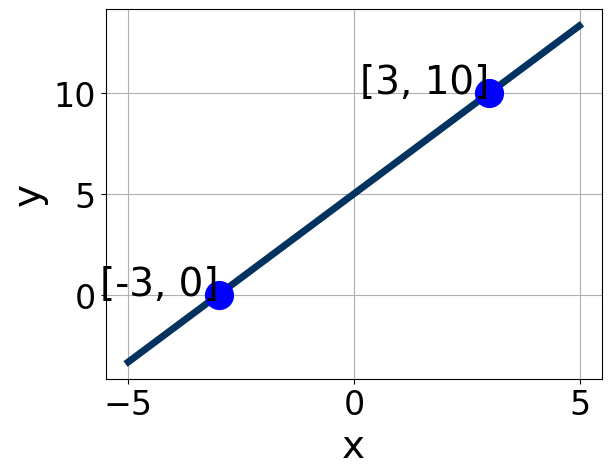
\includegraphics[width=0.5\textwidth]{../Figures/linearGraphToStandardCopyA.png}
\end{center}
\begin{enumerate}[label=\Alph*.]
\item \( A \in [4, 13], \hspace{3mm} B \in [-3.31, -1.73], \text{ and } \hspace{3mm} C \in [-17, -12] \)
\item \( A \in [4, 13], \hspace{3mm} B \in [1.78, 3.94], \text{ and } \hspace{3mm} C \in [10, 19] \)
\item \( A \in [-4.67, 0.33], \hspace{3mm} B \in [-1.23, -0.82], \text{ and } \hspace{3mm} C \in [-6, -4] \)
\item \( A \in [-4.67, 0.33], \hspace{3mm} B \in [-0.18, 1.31], \text{ and } \hspace{3mm} C \in [3, 8] \)
\item \( A \in [-5, -3], \hspace{3mm} B \in [1.78, 3.94], \text{ and } \hspace{3mm} C \in [10, 19] \)

\end{enumerate} }
\litem{
Solve the equation below. Then, choose the interval that contains the solution.\[ -2(17x + 14) = -13(-16x -11) \]\begin{enumerate}[label=\Alph*.]
\item \( x \in [-0.51, -0.45] \)
\item \( x \in [-0.71, -0.67] \)
\item \( x \in [0.47, 0.56] \)
\item \( x \in [-0.69, -0.63] \)
\item \( \text{There are no real solutions.} \)

\end{enumerate} }
\litem{
Solve the linear equation below. Then, choose the interval that contains the solution.\[ \frac{4x + 6}{5} - \frac{-7x -8}{6} = \frac{9x -3}{2} \]\begin{enumerate}[label=\Alph*.]
\item \( x \in [0.8, 2] \)
\item \( x \in [-3.5, -1.2] \)
\item \( x \in [5.9, 7] \)
\item \( x \in [-0.1, 0.8] \)
\item \( \text{There are no real solutions.} \)

\end{enumerate} }
\litem{
Write the equation of the line in the graph below in Standard form $Ax+By=C$. Then, choose the intervals that contain $A, B, \text{ and } C$.
\begin{center}
    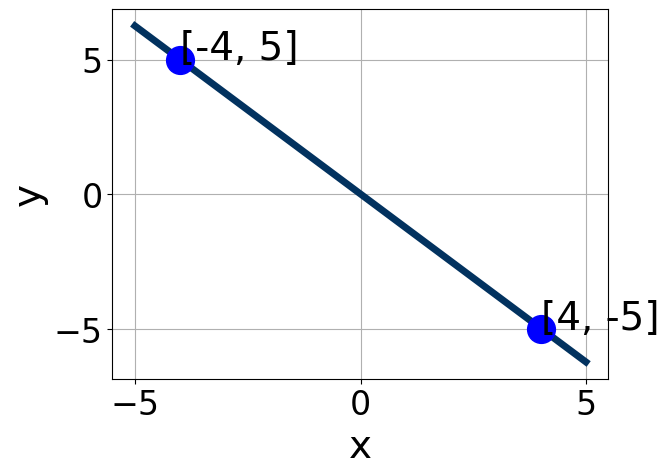
\includegraphics[width=0.5\textwidth]{../Figures/linearGraphToStandardA.png}
\end{center}
\begin{enumerate}[label=\Alph*.]
\item \( A \in [2, 7.8], \hspace{3mm} B \in [-6.3, -3.1], \text{ and } \hspace{3mm} C \in [-4, 3] \)
\item \( A \in [2, 7.8], \hspace{3mm} B \in [3.1, 5.7], \text{ and } \hspace{3mm} C \in [-4, 3] \)
\item \( A \in [-6.7, -4.7], \hspace{3mm} B \in [-6.3, -3.1], \text{ and } \hspace{3mm} C \in [-4, 3] \)
\item \( A \in [-1.2, 3.7], \hspace{3mm} B \in [-1.7, -0.3], \text{ and } \hspace{3mm} C \in [-4, 3] \)
\item \( A \in [-1.2, 3.7], \hspace{3mm} B \in [-0.2, 3.7], \text{ and } \hspace{3mm} C \in [-4, 3] \)

\end{enumerate} }
\litem{
First, find the equation of the line containing the two points below. Then, write the equation as $ y=mx+b $ and choose the intervals that contain $m$ and $b$.\[ (5, -3) \text{ and } (-9, -7) \]\begin{enumerate}[label=\Alph*.]
\item \( m \in [-0.22, 1.37] \hspace*{3mm} b \in [-4.78, -3.52] \)
\item \( m \in [-0.22, 1.37] \hspace*{3mm} b \in [1.97, 2.66] \)
\item \( m \in [-0.22, 1.37] \hspace*{3mm} b \in [3.71, 4.84] \)
\item \( m \in [-0.22, 1.37] \hspace*{3mm} b \in [-9.21, -7.78] \)
\item \( m \in [-0.83, -0.19] \hspace*{3mm} b \in [-10.39, -8.71] \)

\end{enumerate} }
\end{enumerate}

\end{document}